\documentclass[../../main.tex]{subfiles}
\begin{document}

$n\geqq3$ とし，
正 $n$ 角錐の表面を，
底面に含まれない $n$ 個の辺で切り開いて得られる展開図を考える．
正 $n$ 角錐の頂点は，
展開図においては，
異なる $n$ 個の点になっている．
ここでは，
これら $n$ 個の点を通る円の半径が1であるような，
正 $n$ 角錐のみを考えることにする．

\begin{figure}[htbp]
  \centering
  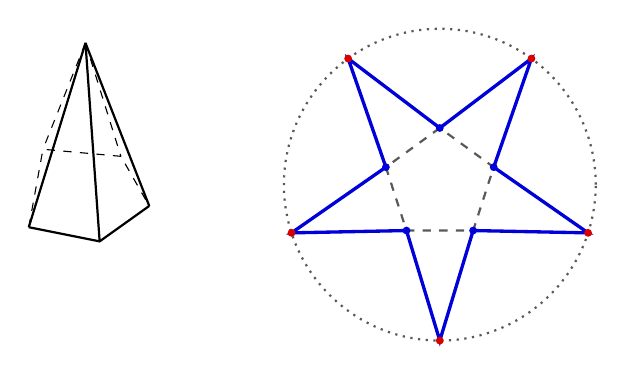
\begin{tikzpicture}[scale=0.9]
    \begin{scope}[shift={(-2.5, 0)}]
      \coordinate (P) at (0, 2);
      \coordinate (A1) at (-0.8, -0.6);
      \coordinate (A2) at (0.2, -0.8);
      \coordinate (A3) at (0.9, -0.3);
      \coordinate (A4) at (0.5, 0.4);
      \coordinate (A5) at (-0.6, 0.5);

      \draw[dashed] (A1) -- (A5) -- (A4) -- (A3);
      \draw[dashed] (P) -- (A5);
      \draw[dashed] (P) -- (A4);

      \draw[thick] (A1) -- (A2) -- (A3);
      \draw[thick] (P) -- (A1);
      \draw[thick] (P) -- (A2);
      \draw[thick] (P) -- (A3);
    \end{scope}

    \begin{scope}[shift={(2.5, 0)}]
      \def\rBase{0.8}
      \def\rApex{2.2}
      \foreach \i in {1,...,5} {
        \coordinate (B\i) at ({90+72*(\i-1)}:\rBase);
        \coordinate (V\i) at ({90+72*(\i-1)+36}:\rApex);
      }
      % 頂点を通る円（半径 1 に対応する円）
      \draw[dotted, thick, gray!70!black] (0, 0) circle (\rApex);
      \draw[dashed, thick, gray!70!black] (B1) -- (B2) -- (B3) -- (B4) -- (B5) -- cycle;

      \draw[very thick, blue!85!black] (B1) -- (V1) -- (B2) -- (V2) -- (B3) -- (V3) -- (B4) -- (V4) -- (B5) -- (V5) -- cycle;
      \foreach \i in {1,...,5} {
        \node[circle, fill=blue!85!black, inner sep=1.0pt] at (B\i) {};
        \node[circle, fill=red!85!black, inner sep=1.0pt] at (V\i) {};
      }
    \end{scope}
  \end{tikzpicture}
\end{figure}

\begin{enumerate}
  \item 各 $n$ に対して，
    このような正 $n$ 角錐の体積の最大値 $v_n$ を求めよ．
  \item $\displaystyle\lim_{n\to\infty}v_n$ を求めよ．
\end{enumerate}

\end{document}
